\documentclass[10pt]{article}
\usepackage[T1]{fontenc}
\usepackage{lmodern,amsmath,amssymb,amsthm,booktabs,microtype}
\usepackage[margin=0.81in]{geometry}
\usepackage[colorlinks=true,urlcolor=blue,linkcolor=blue]{hyperref}
\usepackage{tikz}
\usetikzlibrary{arrows.meta,positioning}
\newtheorem{theorem}{Theorem}
\newtheorem{lemma}{Lemma}
\newtheorem{corollary}{Corollary}
\DeclareMathOperator{\ord}{ord}
\DeclareMathOperator{\Res}{Res}
\DeclareMathOperator{\Norm}{Norm}
\newcommand{\cat}{\mathbin{\Vert}}
\title{Affine Dynamics and Spectral Compression\\
of Decimal Mountain Concatenations}
\author{Qichao Wang}
\date{October 18, 2026 \quad \textit{computer-assisted partial result}}
\begin{document}\maketitle
\begin{abstract}
For \(M(k)=1\cat2\cat\cdots\cat k\cat(k-1)\cat\cdots\cat1\),
we prove that every prime \(p\) with
\(\ord_p(10)=7\cdot2^a5^c\) or
\(\ord_p(10)=11\cdot3^b2^a5^c\), \(a,c\ge0\), \(0\le b\le2\),
divides at least one \(M(k)\).
The argument first compresses the stable affine drift for a
\emph{fixed} coprime-order component \(v\) to at most
\(\ell=\operatorname{lcm}(t,\ord_t(10))\) cyclotomic cosets,
where \(t=v/\gcd(v,9)\),
uniformly over arbitrarily large powers of \(2,5\).
Both drift coordinates become polynomials of degree at most two
in \(m=r/\gcd(r,\ell)\) over a fixed-degree cyclotomic field.
For \(v=11,33,99\), an explicit invariant proves nonzero drift
algebraically when the order is odd; ten fixed norms and a complete
finite sieve settle the even branch. We also give a direct witness
whenever the \(2,5\)-part of the order divides 20, with no restriction
on its coprime part and no nonzero-drift assumption.
This does not resolve the unrestricted OEIS A077187 conjecture.
\end{abstract}

\section{Affine drift and the period reduction}
The primes 2 and 5 never divide a mountain, whose final digit is 1.
The primes 3 and 11 have witnesses \(M(3)=12321\) and \(M(2)=121\).
Unless specified otherwise, the spectral formulas below are for
\(p\ge7\). Set \(r=\ord_p(10)=uv\) with
\(u=2^a5^c\), \((v,10)=1\).
Write \(C_k=1\cat\cdots\cat k\),
\(Y_k=10^{-D(k)}(k\cat\cdots\cat1)\pmod p\),
where \(D(k)\) is the total digit count.
For a complete \(d\)-digit layer, put
\[
L=10^{d-1},\quad q=10^d,\quad n=9L,\quad A=q^n,
\quad S=\sum_{i<n}q^i,\quad J=\sum_{i<n}iq^i.
\]
The exact layer map is
\[
(C,Y)\longmapsto\bigl(AC+(q-1)S-J,\
A^{-1}(Y+LS+J)\bigr).
\]
We will prove that a stable block of \(T\) digit layers is a translation
of displacement \((U,V)\). Consequently its successive end states satisfy
\[
(C_{10^{jT}-1},Y_{10^{jT}-1})
=(C_{10^T-1},Y_{10^T-1})+(j-1)(U,V),\qquad j\ge1.
\]
If \((U,V)\ne(0,0)\), the normalized residues of
\(M(10^{jT})\), \(M(10^{jT}+1)\) have affine slopes
\(10U+V\) and \(1000U+V\). For \(p\ge7\), \(p\ne11\),
these cannot both vanish, yielding a divisible mountain with
\(1\le j\le p\).

Set \(\delta=\gcd(v,9)\), \(t=v/\delta\),
\(b_0=9/\delta\), and \(h=\ord_t(10)\), with \(\ord_1(10)=1\).
Define
\[
\ell=\operatorname{lcm}(t,h),\qquad
g=\gcd(r,\ell),\qquad m=r/g,\qquad T=m\ell.
\]
The key point is that \(\ell\) depends only on \(v\), not on \(a,c\).
Also \(T\ge r\ge\max(a,c)\), so the block starting at \(T+1\)
is in the stable range.

\begin{lemma}[Reduced short-period phase]\label{lem:phase}
For every stable digit layer \(d\), the diagonal multiplier
\(A_d=10^{9d10^{d-1}}\) has period \(\ell\).
Furthermore \(\prod_{j=d}^{d+\ell-1}A_j=1\pmod p\).
Thus its cumulative phase \(P_d\), started at \(d=T+1\),
also has period \(\ell\). The stable multipliers generate precisely
the subgroup of order \(t\).
\end{lemma}
\begin{proof}
Take \(d\) large enough that \(u\mid10^{d-1}\).
Let \(\zeta=10^m\), of order \(g\), and let
\(\eta=u^{-1}\pmod t\). Since \(t\mid g\), division of the
integer exponent by \(u\delta\) gives
\[
A_d=\zeta^{(g/t)b_0\eta\,d10^{d-1}}.
\]
For \(t=1\), read this as \(A_d=1\).
Periodicity follows from \(t\mid\ell\) and \(10^\ell=1\pmod t\).
For the product it suffices to prove
\(E_\ell=\sum_{j=1}^{\ell}j10^{j-1}=0\pmod t\).
Away from 3 this follows from
\(81E_\ell=1+(9\ell-1)10^\ell\).
For the 3-part, induction gives \(s\mid E_s\) when \(s=3^n\):
as \(10^s=1\pmod{3s}\),
\[
E_{3s}=\sum_{k=0}^2 10^{ks}
 \left(E_s+ks\sum_{j=1}^s10^{j-1}\right)
 \equiv3E_s\equiv0\pmod{3s}.
\]
Partitioning any multiple of \(s\) into length-\(s\) blocks gives
the required divisibility. A shifted length-\(\ell\) sum also
vanishes: the extra geometric sum \((10^\ell-1)/9\) is divisible
by \(t\), using \(v_3(10^\ell-1)=2+v_3(\ell)\) at 3.
Finally \((b_0\eta,t)=1\), so \(A_{T+1}\) has order \(t\).

Since \(r\mid T\), the parameters \(q,L\) repeat after \(T\);
the phases do too, and their product in \(T=m\ell\) layers is 1.
The layer maps therefore repeat, with a translation as their block
map. This proves the asserted affine block identity.
\end{proof}

\begin{figure}[h]
\centering
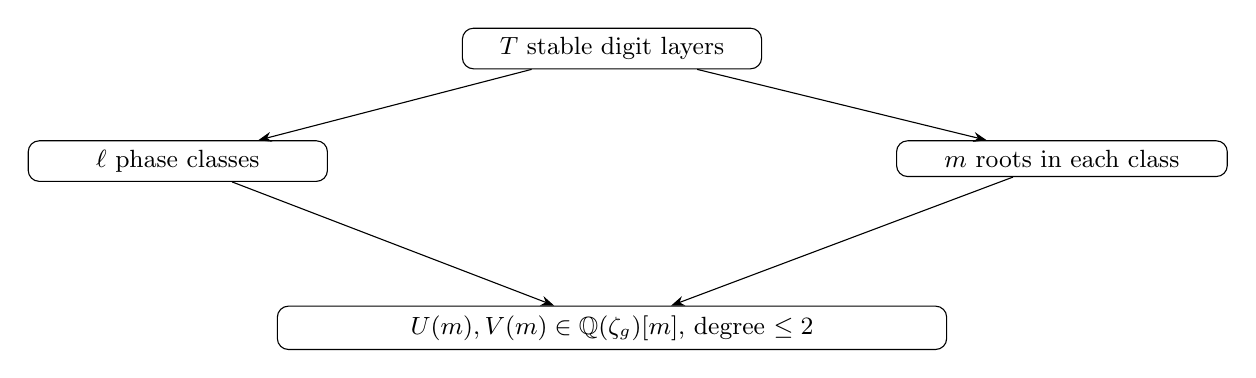
\begin{tikzpicture}[>=Stealth,node distance=7mm,
 every node/.style={font=\small}]
\node[draw,rounded corners,minimum width=38mm] (top)
  {\(T\) stable digit layers};
\node[draw,rounded corners,below left=9mm and 17mm of top,
minimum width=38mm] (lanes)
  {\(\ell\) phase classes};
\node[draw,rounded corners,below right=9mm and 17mm of top,
minimum width=42mm] (orbits)
  {\(m\) roots in each class};
\node[draw,rounded corners,below=13mm of top,
yshift=-17mm,minimum width=85mm] (out)
  {\(U(m),V(m)\in\mathbb Q(\zeta_g)[m]\), degree \(\le2\)};
\draw[->] (top)--(lanes);
\draw[->] (top)--(orbits);
\draw[->] (lanes)--(out);
\draw[->] (orbits)--(out);
\end{tikzpicture}
\caption{The unbounded stable block compresses to bounded-dimensional
cyclotomic algebra once \(v\) is fixed.}
\end{figure}

\section{Coset sums and quadratic spectral coordinates}
Let \(\zeta=10^m\pmod p\), a primitive \(g\)-th root.
For \(j=1,\ldots,\ell\), all layers
\(d=T+j+t\ell\) (\(0\le t<m\)) share the same
\(A=A_j\) and \(P=P_j\). Their values \(q=10^d\)
are precisely the \(m\) roots of \(z^m=c=\zeta^j\).
Define
\[
F_1=\sum_{\substack{z^m=c\\z\ne1}}\frac z{z-1},
\qquad
F_2=\sum_{\substack{z^m=c\\z\ne1}}\frac z{(z-1)^2}.
\]
Logarithmic differentiation of \(z^m-c\), with \(z=1\)
removed if necessary, gives
\[
\begin{array}{c|cc}
 &F_1&F_2\\\hline
c\ne1&mc/(c-1)&m^2c/(c-1)^2\\
c=1&(m-1)/2&-(m^2-1)/12 .
\end{array}
\]
For a nonsingular full layer, its ascending and descending
block residues are
\[
\begin{aligned}
B&=(A-1)\bigl(1+q/(q-1)^2\bigr)-9LA/(q-1),\\
R^*&=(A-1)\bigl(L/(q-1)-q/(q-1)^2\bigr)
 +9LA/(q-1).
\end{aligned}
\]
The singular layer \(q=1\) contributes
\(B=R^*=9/200\). Put
\(\alpha=P^{-1}(1-A^{-1})\),
\(\beta=P(A-1)\), \(n_0=m-\mathbf 1_{c=1}\).

\begin{theorem}[Bounded-degree spectral compression]
For each fixed \(v\), the drift equals the sum of \(\ell\)
coset contributions
\[
\begin{aligned}
U_j&=\alpha(n_0+F_2)-\tfrac9{10}P^{-1}F_1
       +\mathbf1_{c=1}\tfrac9{200}P^{-1},\\
V_j&=\beta(F_1/10-F_2)+\tfrac9{10}PAF_1
       +\mathbf1_{c=1}\tfrac9{200}P.
\end{aligned}
\tag{1}
\]
Moreover,
\[
A_j=\zeta^{(g/t)b_0\eta\,j10^{j-1}},
\quad
P_j=\prod_{s<j}A_s,\quad \eta=u^{-1}\pmod t,
\]
so \(U,V\) are polynomials of degree at most two in \(m\),
with coefficients in the fixed cyclotomic field
\(\mathbb Q(\zeta_g)\), where \(g\le\ell\).
\end{theorem}
\begin{proof}
In the ascending long word the \(j\)-th layer block has weight
\((PA)^{-1}\), while the descending block has weight \(P\).
Substitute the two block residues, sum over the \(m\) roots in
each phase class, and include the singular contribution.
The displayed formulas follow. Their only dependence on \(m\)
is through \(m,m^2\), while all phases are powers of \(\zeta_g\).
\end{proof}


\begin{lemma}[Involutive degree drop for \(\ord_v(10)\le2\)]
If \(v\mid99\), then the coefficients of \(m^2\) in
both compressed drift coordinates vanish identically:
\(U_2=V_2=0\) in the cyclotomic coefficient field.
\end{lemma}
\begin{proof}
For \(v=1\), all stable multipliers equal 1.
Otherwise \(10^2\equiv1\bmod v\) implies
\(A_{-j}=A_j^{-1}\). Because
\(\prod_{j=1}^{\ell}A_j=1\), this yields the
palindrome \(P_{\ell+1-j}=P_j\).
Hence both phase differences
\(\alpha_j=P_j^{-1}-P_{j+1}^{-1}\) and
\(\beta_j=P_{j+1}-P_j\) change sign
under \(j\mapsto\ell-j\).
The coefficient of \(m^2\) in \(F_2\) is the
inversion-even function \(f(c)=c/(c-1)^2\)
for \(c\ne1\), extended by \(f(1)=-1/12\).
Thus \(U_2=\sum_j\alpha_jf(\zeta^j)\) and
\(V_2=-\sum_j\beta_jf(\zeta^j)\)
cancel pairwise under the involution.
\end{proof}

\section{Explicit linear coordinates for coprime parts 11, 33, 99}
Write
\[
r=11w,\quad w=3^b2^a5^c,\quad 0\le b\le2,\qquad
\gamma=w^{-1}\pmod{11}.
\]
Lemma~\ref{lem:phase} gives \(t=11,\ell=22\), with
\(g=11\) if \(a=0\) and \(g=22\) otherwise.
Set \(\omega=\zeta^{g/11}\) and \(\tau=\omega^{9\gamma}\).
The phases satisfy
\[
A_j=\omega^{9\gamma j(-1)^{j-1}},\qquad
P_{2n}=\tau^n,\qquad P_{2n+1}=\tau^{-n}.
\]
In particular \(\sum_{j=1}^{22}P_j=0\). The factor \(3^b\)
must be included in \(\gamma\); discarding it changes the actual phase.

Define \(X(c)=c/(c-1)\) for \(c\ne1\), with \(X(1)=1/2\).
Inversion gives \(X(c^{-1})=1-X(c)\). The phase palindrome and
formula (1) yield
\[
U_1=-\frac9{10}\sum_jP_j^{-1}X(\zeta^j),\qquad
V_1=-\frac{11}{10}\sum_jP_jX(\zeta^j).
\]
The finite Fourier sums needed to evaluate these expressions are
\[
\begin{aligned}
\sum_{c^{11}=1}c^A X(c)&=11/2-A &&(0\le A\le10),\\
\sum_{c^{11}=-1}c^A X(c)&=11/2 &&(0\le A\le10),\\
\sum_{c^{11}=-1}c^{-A}X(c)&=-11/2 &&(1\le A\le10).
\end{aligned}
\]
For the first identity, inverse pairing gives the value at \(A=0\),
and each successive difference is \(-1\), by the root power sums.
For the second, logarithmic differentiation of \(x^{11}+1\) gives
the initial value and the successive differences vanish. The third
follows by multiplying by \(c^{11}=-1\).

\begin{theorem}[Odd branch: a nonzero algebraic invariant]
Every prime with \(r=11\cdot3^b5^c\), \(0\le b\le2\), has nonzero drift.
\end{theorem}
\begin{proof}
Here \(g=11\). Choose \(A\in\{1,\ldots,10\}\) with
\(2A=9\gamma\pmod{11}\), and put \(z=\zeta^A\), \(D=11-2A\).
The even phase indices have \(P=c^A\), the odd ones \(P=zc^{-A}\).
The Fourier sums, together with the singular classes \(j=11,22\), give
\[
\begin{aligned}
U&=\frac{99}{200}(1+z^{-1})+\frac{9D}{20}m(1-z^{-1}),\\
V&=-\frac{81}{200}(1+z)-\frac{11D}{20}m(1-z).
\end{aligned}
\]
Their linear terms cancel in
\[
\boxed{11zU-9V=\frac{909}{100}(z+1).}
\]
Since \(z\) has order 11, \(z+1\ne0\). The prime factors of
\(909=9\cdot101\) are inadmissible: the orders of 10 modulo 3 and
101 are 1 and 4. Thus the right side is nonzero. No norm certificate
is needed in this branch.
\end{proof}

For \(g=22\), take instead \(A=9\gamma\pmod{11}\) in
\(\{1,\ldots,10\}\), with \(z=\zeta^A\), \(D=11-2A\).
Even and odd indices now traverse \(c^{11}=1\) and \(c^{11}=-1\).
The same sums and the single singular class give
\[
U=\frac{99}{200}+\frac{9m}{20}(D-11z^{-1}),\qquad
V=-\frac{81}{200}-\frac{11m}{20}(D-11z).
\]
Consequently
\[
4000z(U_1V_0-U_0V_1)=9(891+40Dz-1331z^2).
\tag{2}
\]
This necessary common-root obstruction uses no division by either
slope, so it remains valid when a slope vanishes modulo \(p\).
The order \(n_A\) of \(z\) is 22 for odd \(A\), and 11 for even \(A\).
Define the ten fixed integers
\[
N_\gamma=\left|\Res_x\bigl(9(891+40Dx-1331x^2),\Phi_{n_A}(x)\bigr)\right|.
\tag{3}
\]
These are exactly the existing even-branch \(v=11\) norms; multiplying
by the root of unity \(z\) does not change their absolute norm.

\begin{theorem}[Even branch: complete exact certificate]
Every prime with \(r=11\cdot3^b2^a5^c\), \(0\le b\le2\),
\(a\ge1,c\ge0\), has nonzero drift.
\end{theorem}
\begin{proof}
All ten integers (3) are nonzero, as checked by exact resultants in
\texttt{certify\_involutive\_families.py}. Simultaneous zero drift would
force \(p\mid N_\gamma\), since (2) vanishes at a primitive
\(n_A\)-th root in \(\mathbb F_p\). Also
\[
r<p\le N_\gamma,\qquad p\mid\Phi_r(10).
\]
The script enumerates every \((a,b,c)\) with
\(11\cdot3^b2^a5^c\le\max_\gamma N_\gamma\), and checks the actual
phase-dependent bound \(r\le N_\gamma\) at each triple. Modular evaluation uses
\[
\Phi_r(X)=\Phi_{22\,3^{[b>0]}5^{[c>0]}}
 \left(X^{2^{a-1}3^{\max(b-1,0)}5^{\max(c-1,0)}}\right).
\]
Every prime dividing the substitution exponent already divides the base
index, so this identity follows by identifying the primitive roots.
The base polynomial has degree at most 80. The complete computation gives
\[
\begin{array}{c|rrr}\toprule
b&0&1&2\\\midrule
\text{Admissible indices}&3887&3796&3702\\
\gcd(N_\gamma,\Phi_r(10))&1&1&1\\\bottomrule
\end{array}
\]
Each raw gcd and each count is asserted. Thus all 11385 possibilities
are excluded. The bound comes from a necessary norm divisor condition;
it is not a cutoff in the desired infinite family.
\end{proof}

\begin{corollary}
Every prime whose order has coprime-to-10 part dividing 99 divides some
\(M(k)\). The branches \(11\mid v,\ a\ge1\) are computer-assisted;
the remaining branches have algebraic proofs.
\end{corollary}
\begin{proof}
For \(v\mid9\), Lemma~\ref{lem:phase} gives \(A=P=1\) and \(T=r\).
Each regular layer contributes \(U+V=0\); the unique \(q=1\) layer
contributes \(9/100\ne0\). For \(v=11,33,99\), use the two theorems.
The two-offset argument gives a witness with \(1\le j\le p\).
The primes 3 and 11 were handled directly.
\end{proof}

\section{The existing quadratic family with coprime part seven}
For \(v=7\), \(h=6\), \(\ell=42\), and
\(g=7\) if \(a=0\), otherwise \(g=14\).
The exact coordinates \(U(m),V(m)\) are quadratic in \(m\).
Their Sylvester resultant
\[
\mathcal R=(U_2V_0-U_0V_2)^2-
  (U_2V_1-U_1V_2)(U_1V_0-U_0V_1)
\]
has, after scaling by \(40000\), a nonzero exact norm,
independent of the six phase values \(\gamma\):
\[
\begin{array}{c|l}
g&|\Norm(40000\mathcal R)|\\\hline
7&33476324853960868807109434619064591936\\
14&114974543608404744933251944861980458578855689
\end{array}
\]
If simultaneous zero drift occurred in this family,
its prime \(p\) would divide the corresponding fixed nonzero
norm \(N\), satisfy \(r=\ord_p(10)\mid p-1\) and
\(p\mid\Phi_r(10)\), hence \(r<p\le N\).
The exact scripts evaluate \(\Phi_r(10)\bmod N\) using
base cyclotomic polynomials of degree at most \(24\)
and modular powering. For all \(53+4479\) admissible indices
in the \(v=7\) norms, they verify that
\(\gcd(N,\Phi_r(10))\) has no prime divisor outside \(r\),
by repeated gcd removal. Since a prime of exact order \(r\)
cannot divide \(r\), zero drift is impossible.
The affine two-offset argument therefore proves existence for every
prime of order \(7\cdot2^a5^c\), without dependence on older smooth-order
certificates.

\section{A direct witness when the smooth part divides 20}
\begin{theorem}[An arbitrary coprime part]
If \(u\mid20\), there is a divisible mountain, regardless of whether
the stable drift vanishes and without restricting \(v\).
\end{theorem}
\begin{proof}
Use the stable period \(T\) above. For every \(d\ge2\),
\(20\mid9d10^{d-1}\), so only the first layer can differ from its
stable continuation. Put \(\alpha=10^9\),
\(\widehat\alpha=10^{9(T+1)10^T}\pmod p\),
and \(\rho=\widehat\alpha/\alpha\). The first-layer map is
\[
C'=\alpha(C+10/81)-91/81,\qquad
Y'=\alpha^{-1}(Y+1/81)+80/81.
\]
Let the stable block be the translation by \(B=(U,V)\).
Its remaining layers have diagonal multiplier
\((\widehat\alpha^{-1},\widehat\alpha)\). Thus the actual first
block ends at \(D+B\), where
\[
D=((\rho^{-1}-1)10/81,\ (\rho-1)/81).
\]
After \(p\) blocks the state is \(D+pB=D\).
Within a \(q\ne1\) window starting at \(L\), the exact recurrence gives
\[
\frac{M(L+n)}{10^{D(L+n-1)}}=qAq^n+B_0q^{-n}-\frac{2q}{(q-1)^2},
\quad
A=C+\frac L{q-1}+\frac1{(q-1)^2},\quad
B_0=Y-\frac L{q-1}+\frac q{(q-1)^2}.
\]
At the window starting at \(10^{pT}\), its modular parameters are
\(q=10,L=1\), giving the square
\[
\frac{(10z-\rho)^2}{81\rho z},\qquad z=10^n.
\]
Choose \(n=(9\cdot10^T-10)\bmod r\), with \(0\le n<r\).
Then \(z=\rho/10\), so \(k=10^{pT}+n\) is a witness. The window
is long enough since \(r<p\). The divisions by 81 are valid for
\(p\ne3\); the case 3 has the direct witness already given.
\end{proof}


\section{The boundary of the short-period mechanism}
Lemma~\ref{lem:phase} also contains the nine-torsion lifting lemma:
for \(v=sv_0\), \(s\mid9\), \((v_0,30)=1\), the reduced phase
component is \(t=v_0\), and its effective phase is \((su)^{-1}\).
If \(3\nmid\ell_0\), the field degree is unchanged. The separate
\texttt{certify\_fixed\_v33\_v99.py} certificate checks 3850 and
3757 indices, including the odd branches now settled algebraically.
Its 15 independent prime-field tests agree with the new formulas.

\begin{lemma}[Exact 3-adic boundary]
Suppose \(r=\ord_p(10)=11\cdot3^b2^a5^c\) with
\(b\ge1\), and set \(A_d=10^{9d10^{d-1}}\) on stable
digit layers. For \(t\ge0\),
\[
\boxed{
\ord(A_{d+22\cdot3^t}/A_d)
=3^{\max(b-2-t,0)}.}
\]
Consequently the 22-period folding is valid
precisely for \(b\le2\) among these 3-power extensions.
\end{lemma}
\begin{proof}
Let \(L=22\cdot3^t\) and \(e_d=9d10^{d-1}\).
The exact difference
\[
e_{d+L}-e_d=
9\cdot10^{d-1}\bigl(L+(d+L)(10^L-1)\bigr)
\]
is divisible by \(11\) and by the smooth factor
\(2^a5^c\) in the stable range.
By the 3-adic lifting-the-exponent lemma,
\(v_3(10^L-1)=2+t\), while \(v_3(L)=t\).
Therefore \(v_3(e_{d+L}-e_d)=2+t\) exactly.
The claimed order follows from
\(\ord_p(10)=11\cdot3^b2^a5^c\).
\end{proof}

This is an obstruction to reusing the 22-phase proof, not an
obstruction to the existence of divisible mountains.

\clearpage
\section{Reproducibility and scope}
The files \texttt{certify\_fixed\_v7.py} and
\texttt{certify\_involutive\_families.py} generate the exact norms and
check every phase-dependent cyclotomic gcd, without factoring
the large norm integers or enumerating target primes.
Independent prime-field tests are in
\texttt{audit\_fixed\_v7.py} and \texttt{audit\_fixed\_v11.py}.
The file \texttt{audit\_reduced\_spectral.py} compares the reduced
phases and explicit cosets with an independent full-layer recurrence.
These finite comparisons check implementation consistency; the universal
identities follow from the proofs above. Dedicated CI jobs reproduce
the certificates. The new linear formulas and exhaustive sieve also
received a separate audit recorded in
\texttt{audit\_spectral\_update\_2026-10-18.md}.
The independent nine-torsion checks are preserved in
\texttt{certify\_fixed\_v33\_v99.py} and
\texttt{audit\_fixed\_v33\_v99.py}.

The spectral theorem applies to arbitrary fixed \(v\), but a
nonzero resultant and the elimination of its actual-order
prime factors are \emph{not} established for arbitrary \(v\).
The general all-primes A077187 problem remains open.

The present proofs impose no restriction on \(v\) when \(u\mid20\),
and no restriction on \(u\) in the certified coprime-part families.
Outside their union, the unresolved question is either to prove nonzero
drift or to force a subgroup root on an actual zero-drift orbit.
The separate note \texttt{zero\_drift\_continuation\_2026-10-18.md}
reduces the first-window tail phase to order \(u/\gcd(u,20)\), but
also shows why three fixed initial windows do not universally suffice.
Those additional reachability results are not assumptions in any of
the existence proofs in this paper.

\begin{thebibliography}{9}
\bibitem{oeis} OEIS Foundation,
\emph{A077187}, \url{https://oeis.org/A077187}.
\bibitem{repo} Q. Wang,
\emph{Decimal mountain concatenation research notes and exact certificates},
\url{https://github.com/dongxuelian2/oeis-papers/pull/8}, 2026.
\end{thebibliography}
\end{document}
